\chapter{Аналитический раздел}
\label{cha:analytical}
\par В данном разделе приведен анализ предметной области: рассмотрены существующие решения поставленной задачи, проведена формализация объектов синтезируемой сцены, приведен обзор существующих методов и алгоритмов для решения поставленной задачи.

	\section{Обзор существующих решений}
	\par На рисунке \ref{pic:galaxy3d} показана модель солнечной системы в программе Galaxy3D. Эта программа позволяет пользователям наблюдать за солнечной системой в движении, но не позволяет контролировать ход времени в программе. Также у пользователей имеется возможность просмотреть информацию о планете, кликнув на нее. Данная программа является одной из самых популярных в сфере симуляции движения планет. [\ref{bib:2}]
	\begin{figure}[h!]
        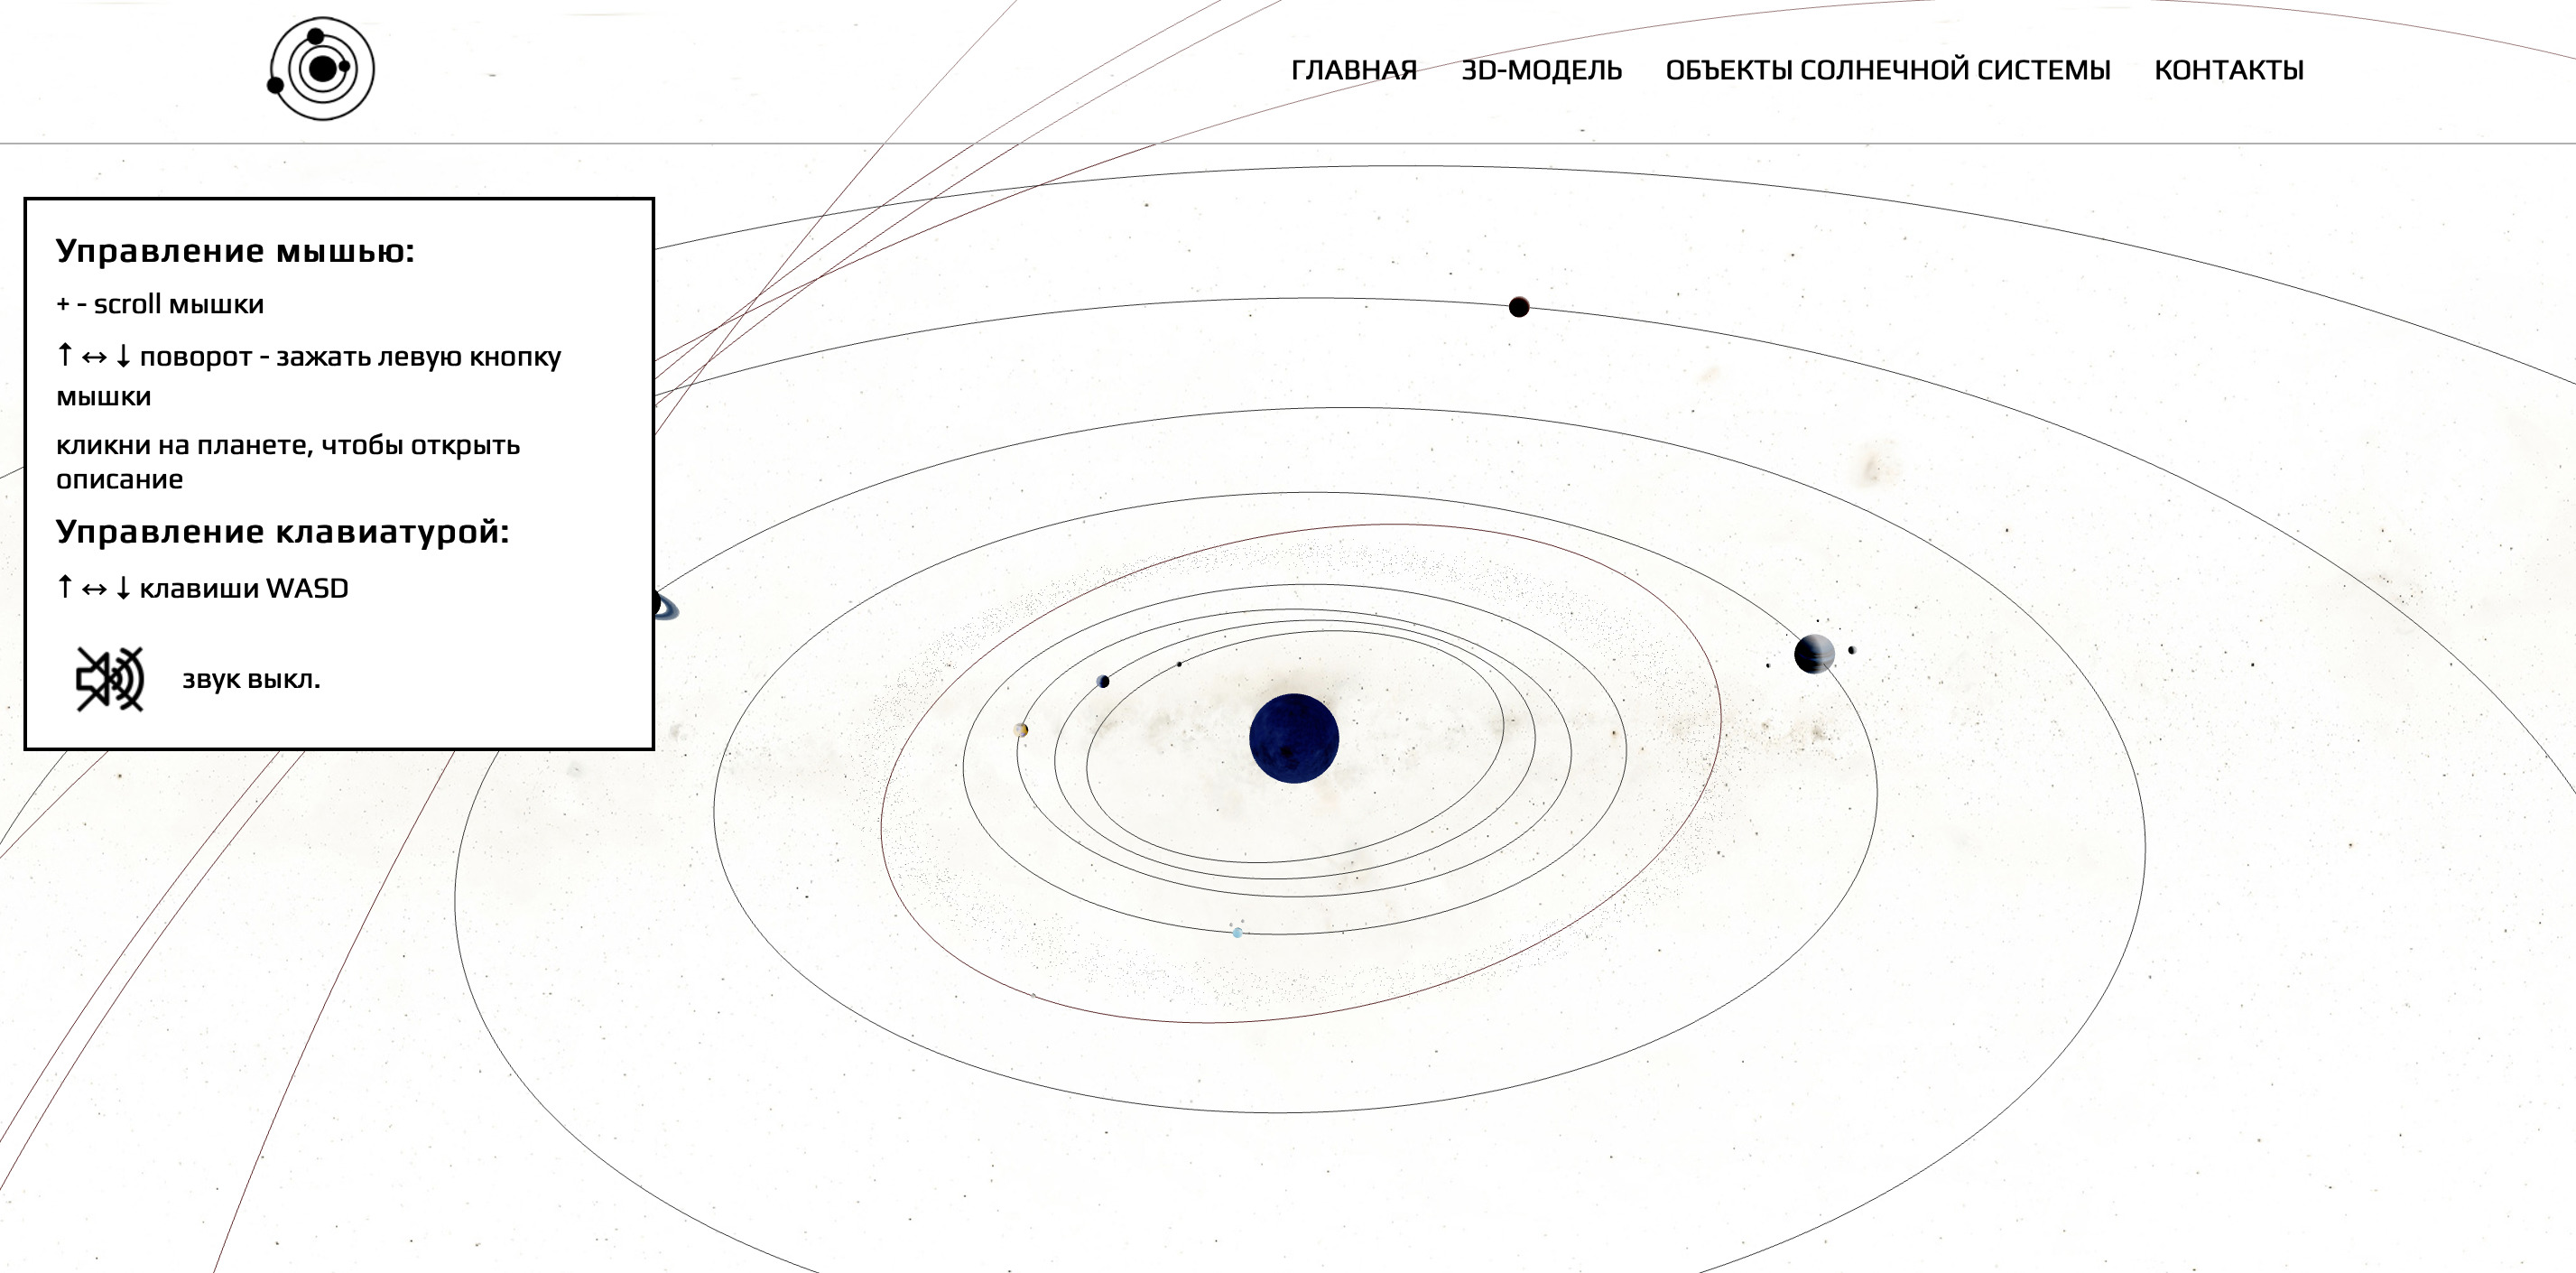
\includegraphics[scale=0.35]{inc/SpaceGid.jpg}
        \caption{Модель солнечной системы в Galaxy3D}
        \label{pic:galaxy3d}
	\end{figure}

	\par На рисунке \ref{pic:spacegid} показана модель солнечной системы в программе SpaceGid. Эта программа, также как и Galaxy3D, позволяет пользователям наблюдать за солнечной системой в движении, но, в отличии от Galaxy3D, она позволяет контролировать ход времени в программе. Функционал в данной программе дает возможность наблюдать за какой-то конкретной планетой, чего пользователь не мог сделать в Galaxy3D. Также имеется возможность контролировать скорость анимации и масштаб планет. [\ref{bib:3}]
	\begin{figure}[h!]
        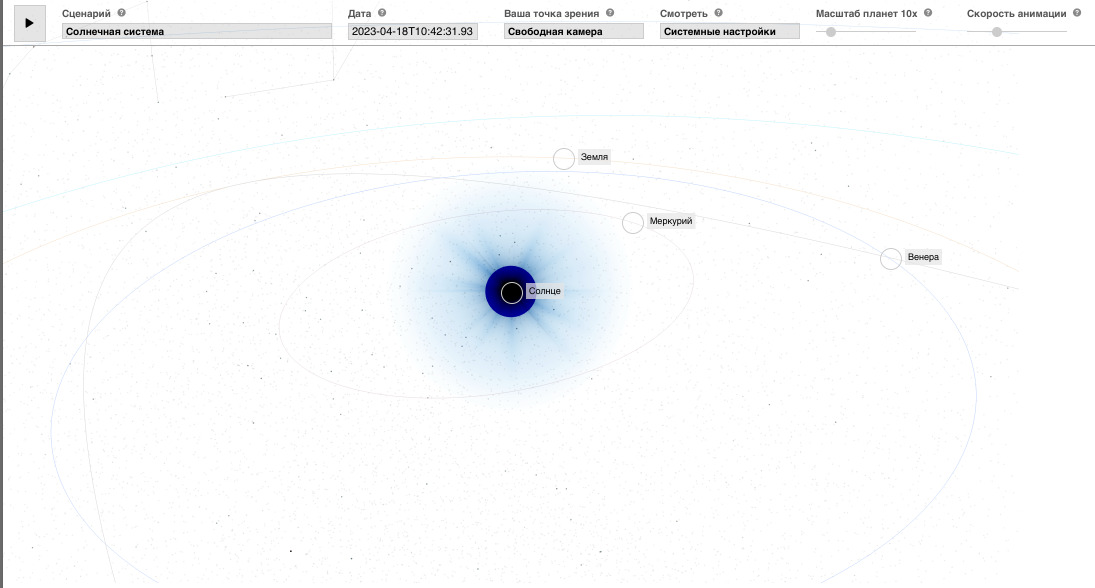
\includegraphics[scale=0.9]{inc/Galaxy3D.jpg}
        \caption{Модель солнечной системы в SpaceGid}
        \label{pic:spacegid}
	\end{figure}

	\par \text{  }
	\par \text{  }
	\par \text{  }
	\section{Формализация объектов сцены}
	\par Сцена состоит из следующих объектов:
	\begin{enumerate}
		\item Звезда -- источник света, который является сферическим объектом;
		\item Планеты -- объект, который является выпуклым симметричным многогранником.
	\end{enumerate}

	\par Ниже представлены характеристики для объектов типа \textbf{Звезда}.
	\begin{enumerate}
		\item Координаты центра масс в экранной СК;
		\item Радиус;
		\item Масса;
		\item Параметр, используемый для вычисления количества узлов для построения полигональной сетки.
	\end{enumerate}

	\par Ниже представлены характеристики для объектов типа \textbf{Планета}.
	\begin{enumerate}
		\item Начальные координаты центра масс;
		\item Текущие координаты центра масс в экранной СК;
		\item Начальная скорость;
		\item Цвет поверхности;
		\item Масса планеты;
		\item Параметр, используемый для вычисления количества узлов для построения полигональной сетки.
	\end{enumerate}

	\section{Анализ способов задания трехмерных моделей}
	Модель можно задать несколькими способами:
	\begin{enumerate}
		\item Каркасная модель -- модель, состоящая из вершин и рёбер, которые определяют форму отображаемого объекта;
		\item Поверхностная модель -- совокупность ограничивающих модель поверхностей, называемых полигонами;
		\item Объемная модель -- модель, состоящая из полигонов. Отличается от поверхностной модели тем, что усточняется информация о материале модели.
	\end{enumerate}

	В таблице \ref{table:ModelCompare} приведено сравнение способов задания трехмерных моделей.

	 \begin{table}[h!]
            \caption{Сравнение способов задания трехмерных моделей}
            \centering
            \begin{tabular}{|l|c|c|c|}
            \hline
            $\text{Характеристика}$ & $\text{КМ}$ & $\text{ПМ}$ & $\text{ОМ}$\\ \hline
            $\text{Применимость к сферическим объектам}$ & нет & да & да\\ \hline
            $\text{Применимость к произвольным выпуклым объектам}$ & нет & да & да\\ \hline
            
            \end{tabular}
            \label{table:ModelCompare}
    \end{table}
    \par Обозначения: КМ -- каркасная модель, ПМ -- поверхностная модель, ОМ -- объемная модель. Для оценки используется
    бинарный признак.  
    \par Для решения поставленной задачи был выбран поверхностный способ задания трехмерных моделей, так как для реализации поставленной задачи не требуется информация о материале модели.

    \section{Алгоритм построения поверхностной модели}
    \par Для хранения информации о полигонах был выбран способ хранения с использованием списка граней. Каждый элемент этого списка представляет из себя список вершин, составляющих данную грань.
    \par В качестве примера будет рассмотрен алгоритм для сферы.
    \par На рисунке \ref{pic:pol_alg} рассматривается сечение сферы плоскоостью \begin{math}OXY\end{math} в экранной СК. Сечение сферы любой плоскостью всегда даст окружность или точку в частном случае.

    \begin{figure}[h!]
    	\begin{center}
        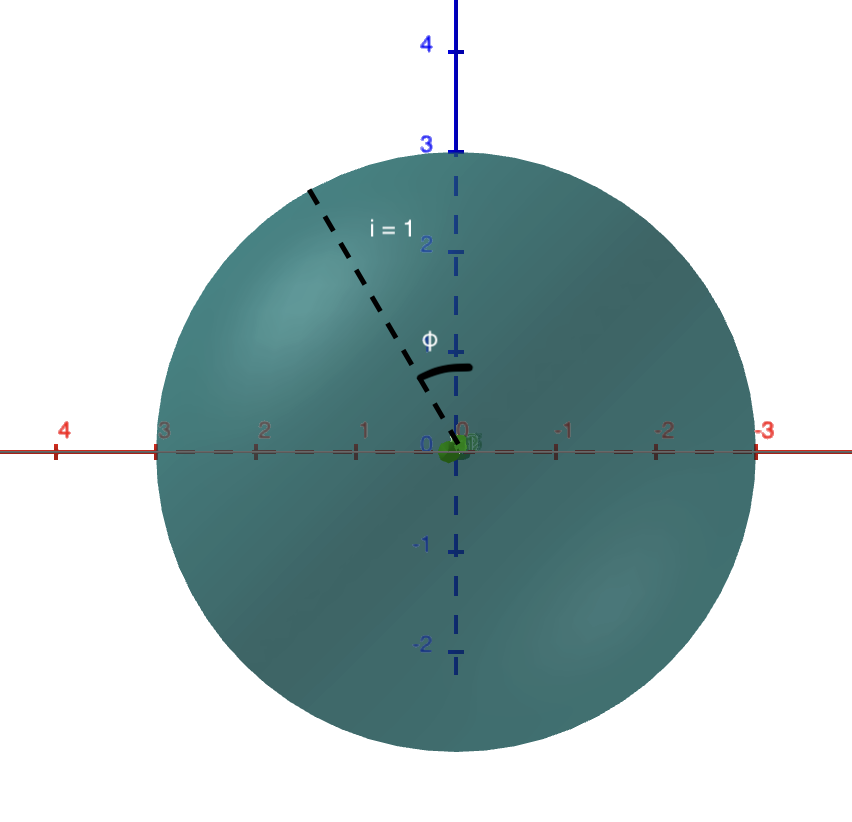
\includegraphics[scale=0.6]{inc/pol_al.png}
        \caption{Сечение сферы плоскостью OXY}
        \label{pic:pol_alg}
        \end{center}
	\end{figure}
    \par Рассмотрим алгоритм генирации вершин полигональной сетки для \begin{math}\frac{1}{4}\end{math} окружности. Остальные вершины можно получить в виду симметрии сферы.
    \par Пусть 
    \begin{enumerate}
    	\item $center$ -- центр сферы
    	\item $R$ -- радиус сферы
    	\item $points$ -- массив вершин полигональной сетки
    	\item $n$ -- параметр, опеределяющий количество вершин между левой и верхней вершинами окружности.
    \end{enumerate}
    \par Таким образом, вычисление $i$-ой вершины сетки \begin{math}\frac{1}{4}\end{math} окружности можно описать следующим образом:
    \begin{equation}\label{formula:Sphere_Alg}
	tmp = \sqrt{2\cdot R^2 \cdot \left( 1 - \left( \cos{\frac{90}{n+1} \cdot i}\right) \right)},
	\end{equation}
	\begin{equation}\label{formula:Sphere_Alg_1}
	dx = \sin{\left( \frac{90}{n+1} \cdot i \right)} \cdot R,
	\end{equation}
	\begin{equation}\label{formula:Sphere_Alg_2}
	dy = \sqrt{tmp^2 - dx^2},
	\end{equation}
	\begin{equation}\label{formula:Sphere_Alg_3}
	point_i = (center_x - dx, center_y + R - dy, center_z).
	\end{equation}
	\par Для получения полной сетки необходимо:
	\begin{enumerate}
		\item получить набор вершин для верхней полуокружности;
		\item произвести серию поворотов полуокружности относительно оси \begin{math}OX\end{math} с шагом, равным \begin{math}\frac{90}{n+1}\end{math}. Результат каждого поворота -- набор вершин, определяющих очередную полуокружность;
		\item на основе списка вершин создается список граней. Для каждого полигона в этом списке хрантся не сами вершины, а их индексы в массиве вершин, что значительно экономит ресурсы. [\ref{bib:4}]
	\end{enumerate}
	\par Таким образом можно создавать не только сферы, но и любые другие симметричные выпуклые фигуры.

	\section{Анализ алгоритмов удаления невидимых ребер и поверхностей}
	\par В поставленной задаче требуется создать анимацию движения планет, следовательно время -- наиболее важный ресурс. Таким образом алгоритм удаления невидимых ребер и поверхностей должен обладать характеристикой быстродействия.

	\subsection{Алгоритм Варнока}
	\par Данный алгоритм работает в пространстве изображений.
	\par Сцена является начальным окном. Затем, алгоритму требуется определить, что изображать в очередном окне. Если нельзя однозначно ответить на этот вопрос, то окно делится на два. Так продолжается либо пока не достигнут предел в один пиксель, либо пока окно не будет закрашено.
	\par Существуют возможные оптимизации данного алгоритма: сортировка многоугольников по координате $z$ и хранение информации о многоугольниках. Данные оптимизации помогают увеличить быстродействие алгоритма, но они создают другую проблему -- увеличение затрачиваемой памяти. [\ref{bib:5}]
	\par Особенностями этого алгоритма являютмя возможность устранить лестничный эффект, рекурсивный вызов и недостаточная быстродейственность.

	\subsection{Алгоритм Z-буфера}
	\par Данный алгоритм работает в пространстве изображений, используя буфер
кадра для заполнения интенсивности каждого пикселя, здесь вводится
некоторый $Z$-буфер (буфер глубины каждого пикселя).
	\par Значение каждого нового пикселя, который нужно занести в буфер кадра,
сравнивается с глубиной пикселя, занесенного в $Z$-буфер. Если сравнение
показывает, что новый пиксель расположен ближе к наблюдателю, то новое
значение $z$ заносится в буфер и корректируется значение интенсивности.
	\par Алгоритм, использующий $Z$-буфер крайне прост в своей реализации по
сравнению с другими анализируемыми алгоритмами, также не тратится время
на сортировку элементов сцены.
	\par Но несмотря на его быстродействие увеличиваются затраты по памяти при
использовании данного алгоритма, запоминается информация по каждому
пикселю изображения. [\ref{bib:6}]
\par Вычислительная сложность данного алгоритма равна 
\begin{math}
O(n\cdot m\cdot k)
\end{math}, где
\begin{math}
n\cdot m
\end{math} –
количество пикселей в буфере кадра, $k$ – количество полигонов.
\subsubsection*{Алгоритм}
\begin{enumerate}
	\item  Всем элементам буфера кадра присвоить фоновое значение;
	\item Инициализировать Z-буфер минимальными значениями глубины;
	\item Выполнить растровую развертку каждого многоугольника сцены:
	\begin{enumerate}
		\item   Для каждого $i$-го пикселя, связанного с многоугольником вычислить его
глубину \begin{math}
z(x_i, y_i)
\end{math};
		\item  Сравнить глубину пикселя со значением, хранимым в Z-буфере. Если
\begin{math}
z(x_i, y_i)
\end{math} > \begin{math}
z_b(x_i, y_i)
\end{math}, то \begin{math}
z_b(x_i, y_i)
\end{math} = \begin{math}
z(x_i, y_i)
\end{math} и цвет\begin{math}
(x_i, y_i)
\end{math} = цвет $i$-го пикселя;
	\end{enumerate}
\end{enumerate} 
\subsubsection*{Математические основы алгоритма}
При известном уравнении плоскости, несущей конкретный многоугольник,
вычисление глубины каждого пикселя могут быть произведены пошаговым
способом.
\par Уравнение плоскости имеет следующий вид (выражено через $z$):
\begin{equation}
		z = \frac{
		ax + by + d
  		}{
  		c
		}
 		\neq 0,
\end{equation}
где $a$, $b$, $d$, $c$ -- коэффициенты уравнения.
\par Для сканирующей строки \begin{math} y =\end{math} const, глубина пикселя, у которого \begin{math} x_1 = x + \Delta x\end{math}, поэтому равна:
\begin{equation}
		z_1 - z = - \frac{
		ax_1 +d
  		}{
  		c
		}
 		+  \frac{
		ax +d
  		}{
  		c
		} = 
 		\frac{
		a(x - x_1)
  		}{
  		c
		},
\end{equation}
\par Отсюда получаем, что
\begin{equation}
		z_1 = z - \frac{
		a
  		}{
  		c
		}\Delta x
	\text{, } 
		\Delta x = 1
	\text{, поэтому } 
		z_1 = z - \frac{
		a
  		}{
  		c
		}.
\end{equation}
\par Поскольку в данной задаче для визуализации используется только один вид
многоугольников, а именно треугольник, то нахождение абсцисс точек
пересечения горизонтали со сторонами треугольника будет выглядеть
следующим образом:
\begin{enumerate}
	\item Для каждой из сторон треугольника будут записываться параметрические
уравнения вида:
	\begin{equation}
		x = x_H + (x_K - x_H)t,
	\end{equation}
	\begin{equation}
		y = y_H + (y_K - y_H)t,
	\end{equation}
	\item После этого для каждой стороны находится параметр \begin{math} t \end{math}при пересечении с горизонталью \begin{math} y = c\end{math}:
	\begin{equation}
		c = y_H + (y_K - y_H)t
	\text{, где } 
		t = \frac{
		c - y_H
  		}{
  		y_K
		} - y_H
	\end{equation}
	\item Если \begin{math} t \in (0, 1)\end{math} , то рассчитывается абсцисса точки
пересечения горизонтали со стороной треугольника:
	\begin{equation}
		x = x_H + (x_K - x_H) \frac{
		c - y_H
  		}{
  		y_K - y_H
		}
	\end{equation}
	\begin{figure}[h!]
		\center{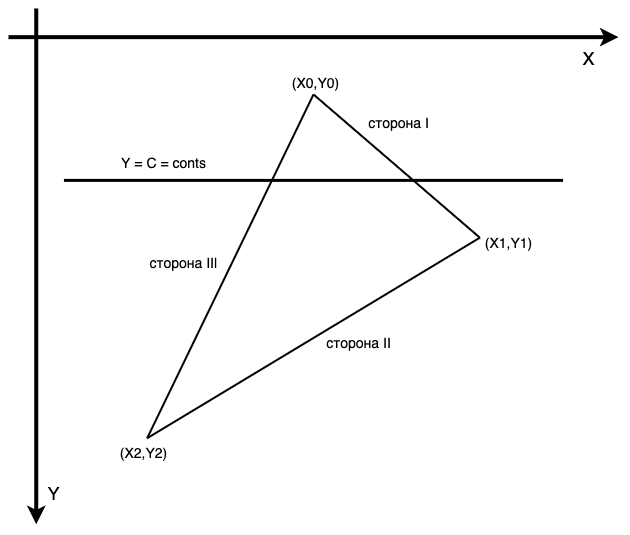
\includegraphics[width=0.6\linewidth]{inc/z.png}}
		\caption{Поиск абсцисс точек пересечения}
		\label{ris:image_z}
	\end{figure}
\end{enumerate}
\par Особенностями алгоритма являются возможность работы со сценами любой сложности, отсутствие требования предварительной сортировки объектов по глубине, сравнительно большой объем затрачиваемой памяти, возникновение лестничного эффекта.

	\subsection{Алгоритм Робертса}
	\par Алгоритм работает только с выпуклыми телами. Если тело изначально является невыпуклым, то предварительно его нужно разбить на выпуклые составляющие. [\ref{bib:6}]
	\par Ниже приведены основные этапы работы алгоритма.
	\begin{enumerate}
		\item[0)] Подготовка исходных данных;
		\item Удаление рёбер или граней, экранируемых самим телом;
		\item Удаление рёбер, экранируемых другими телами;
		\item Вычисление отрезков, которые образуют новые ребра при протыкании других объектов друг друга.
	\end{enumerate}
	\par Особенностями алгоритма является высокая точность вычислений, невозможность работы с прозрачными и просвечивющими объектами, невозможность передачи падающих теней, метод строго ориентирован на выпуклые многогранники. [\ref{bib:13}]
	\subsubsection*{Вывод}

	\par В таблице \ref{table:OtrCompare} приведено сравнение алгоритмов удаления ребер и поверхностей.

	 \begin{table}[h!]
            \caption{Сравнение алгоритмов удаления ребер и поверхностей}
            \centering
            \begin{tabular}{|l|c|c|c|}
            \hline
            $\text{Характеристика}$ & $\text{АВ}$ & $\text{АБ}$ & $\text{АР}$\\ \hline
            $\text{Скорость вычислений}$ & \begin{math} O(S_{pic}\cdot n) \end{math} & \begin{math} O(S_{pic}\cdot n) \end{math} & \begin{math} O(n^2)\end{math}\\ \hline
            $\text{Применимость к произвольным выпуклым объектам}$ & да & да & да\\ \hline
            $\text{Объемные вычислительные затраты}$ & да & нет & да\\ \hline
            \end{tabular}
            \label{table:OtrCompare}
    \end{table}
    \par Обозначения: АВ -- алгоритм Варнока, АБ -- алгоритм $Z$-буфера, АР -- алгоритм Робертса.
    \par Для решения поставленной задачи был выбран алгоритм $Z$-буфера.

    \section{Анализ методов и алгоритмов закрашивания}
   	\par Главное требование, выдвигаемое к алгоритму закраски в рамках поставленной задачи, также как и в разделе выше, -- быстродействие. [\ref{bib:8}]

   	\subsubsection*{Типы источников света}
   	\par Основные типы источников света: точечные, прожекторы и бесконечно удаленные (направленные).
   	\par В посталвенной задаче Звезда не является точетным источником света. Также Звезда не является направленным источником света, так как в задаче не допускается считать её лучи параллельными. При этом Звезда не является прожектором, так как она не излучает свет конусом.
   	\par Поверхность Звезды будет рассматриваться как множество точечных источников.

   	\subsection*{Модели освещения}
   	\par Существует два типа моделей освещения, используемых в синтезе трехмерных изображений: локальная модель освещения и глобальная модель освещения. Модель называется локальной, если не учитывает перенос света между поверхностями. Иначе модель называют глобальной. Далее будут рассмотреты только локальные модели освещения, поскольку для частой смены кадров важна производительность.

   	\subsubsection*{Простая модель освещения}
   	\par Модель Ламберта моделирует идеальное диффузное освещение.
   	\par Интенсивность освещенности точки в этой модели находится по закону Ламберта:
   	\begin{equation}\label{formula:Lambert}
		I_{d} = I_0 \cdot \cos{(\alpha)},
	\end{equation}
	\par где \begin{math}I_{d}\end{math} -- уровень освещенности в ассматриваемой точке, \begin{math}I_0\end{math} -- максимальный уровень освещенности, \begin{math}\alpha\end{math} -- угол между вектором нормали к плоскости и вектором, направленным от рассматриваемой точки к источнику освещения.
	\begin{figure}[h!]
		\center{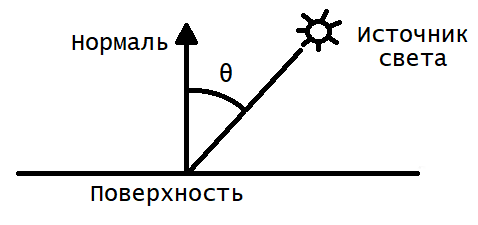
\includegraphics[width=0.49\linewidth]{inc/light.png}}
		\caption{Простая модель освещения}
		\label{ris:image_l}
	\end{figure}

	\subsubsection*{Модель освещения по Фонгу}
	\par Свет в модели освещения Фонга состоит из нескольких составляющих:
	\begin{itemize}
		\item Диффузная (рассеянная) -- рассчитывается по закону Ламберта (\ref{formula:Lambert}), исходя из предположения, что при попадании наповерхность свет рассеивается равномерно во все стороны;
		\item Окружающая (фоновая) -- некоторая константа, которая прибавляется к освещенности в каждой точке освещаемой модели;
		\item Зеркальная -- придает объектам блеск.
	\end{itemize}
	\par Итоговая формула освещенности в точке выглядит следующим образом:
	\begin{equation}\label{formula:Fong}
		I = I_{d} + I_{env} + I_{mir},
	\end{equation}
	\par где \begin{math}I\end{math} -- интенсивность в ассматриваемой точке, \begin{math}I_{env}\end{math} -- интенсивность окружающего света, \begin{math}I_{mir}\end{math} -- интенсивность зеркального света.
	\begin{figure}[h!]
		\center{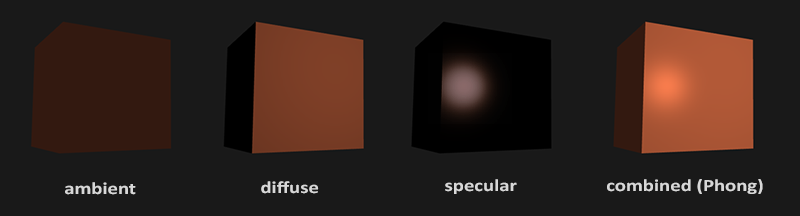
\includegraphics[width=0.49\linewidth]{inc/fong.png}}
		\caption{Модель освещения Фонга}
		\label{ris:image_f}
	\end{figure}
	\par Для учета фоновой составляющей вводят небольшой коэффициент фонового освещения.
	\par Так как планеты не обладают зеркальными свойствами, в рамках поставленной задачи \begin{math}I_{mir} = 0\end{math}.
	\par Так как поверхности планет не обладают зеркальными эффектами, а фоновая составлюща сравнительно мала, было решено использовать простую модель освещения.

	\subsection*{Простая закраска}
	\par Весь полигон закрашивается одним уровнем интенсивности, который вычисляется по закону Ламберта.
	\par При использовании данного метода все плоскости будут закрашены однотонно, и в результате вращения могут возникнуть ложные ребра в виду того, что цвета соседних граней могут сильно отличаться. Этот эффект можно сгладить, если использовать большое число плоскостей.
	\par Данный метод не требователен к ресурсам, и у модели, полученной данным методом, четко видны переходы между полигонами.

	\subsection*{Закраска по Гуро}
	\par Полигон закрашивается не одним цветом, а плавно изменяющимися оттенками одного цвет, вычисляемыми путем интерполяции цветов примыкающих граней.
	\par Основные этапы:
	\begin{enumerate}
		\item для каждой грани вычислется вектор нормали;
		\item вычисляется нормаль каждой вершины как среднее арифметическое между нормалями всех граней, пересекающихся в данной вершине;
		\item рассчитывается интенсивность освещения в вершинах пропорционально косинусу угла между нормалью в вершине и направлением света;
		\item каждый многоугольник закрашивается путем линейной интерполяции значений интенсивностей в вершинах сначала вдоль каждого ребра, а затем и между ребрами вдоль каждой сканирующей строки.
	\end{enumerate}
	\par Закраска по Гуро имеет высокое качество построения зеркальных бликов и матовых поверхностей, но при этом имеет сравнительно большие вычислительные затраты и возможность осуществления ситуации, когда ребро многоугольника при закраске может стать незаметным.

	\subsection*{Закраска по Фонгу}
	\par Данный метод аналогичен закраске по Гуро, однако было предложено интерполиговать не интенсивности в вершинах, а нормали.
	\par Этот метод более трудоемкий, чем аналогичный ему метод закраски по Гуро, описанный выше: для каждой точки поверхности необходимо совершать больше вычислительных операций.
	\par Закраска по Фонгу строит изображения с высоким качеством, особенно для поверхностей с зеркальными свойствами.

	\subsubsection*{Вывод}
	\par В таблице \ref{table:LightCompare} приведено сравнение алгоритмов закрашивания полигонов.
	 \begin{table}[h!]
            \caption{Сравнение алгоритмов закрашивания полигонов}
            \centering
            \begin{tabular}{|l|c|c|c|}
            \hline
            $\text{Характеристика}$ & $\text{ПЗ}$ & $\text{ЗГ}$ & $\text{ЗФ}$\\ \hline
            $\text{Учёт зеркальных и матовых бликов}$ & нет & да & да\\ \hline
            $\text{Высокие вычислительные затраты}$ & нет & да & да\\ \hline
            $\text{Применимость к произвольным выпуклым объектам}$ & да & да & да\\ \hline
            \end{tabular}
            \label{table:LightCompare}
    \end{table}
    \par Обозначения: ПЗ -- алгоритм простой закраски, ЗГ -- алгоритм закраски по Гуро, ЗФ -- алгоритм закраски по Фонгу. 
    \par Для решения поставленной задачи был выбран алгоритм простой закраски т.к. основным критерием для данной задачи является быстродействие.
    \section{Физическая составляющая}
    \par В данной работе требуется реализовать движение планет по физическим законам. 
    \par По закону всемирного тяготения вычисляем силу тяготения в момент времени $t$ для каждого объекта на сцене.
    \begin{equation}\label{formula:F}
		F_i^t = \sum_{j=0}^{n} G \cdot \frac{m_i \cdot m_j}{R_{ij}^2}, j \neq i, 
	\end{equation}
	где $n$ -- количество объектов на сцене, \begin{math}m_i\end{math} -- масса $i$-го объекта, \begin{math}m_j\end{math} -- масса $j$-го объекта, \begin{math}R_{ij}\end{math} -- расстояние между $i$-м и $j$-м объектом. [\ref{bib:14}]
	\par Используя явную схему Эйлера решения дифференциальных уравнений и второй закон Ньютона, скорость в момент времени $t$ вычисляется по формуле (\ref{formula:v}).
	\begin{equation}\label{formula:v}
		\vec{v_i^t} = \frac {F_{i}^{t-1} \cdot dt} {m_i},
	\end{equation}
	где \begin{math}m_i\end{math} -- масса $i$-го объекта, \begin{math}F_{i}^{t-1}\end{math} -- сила тяготения для $i$-го объекта в момент времени $t-1$, \begin{math}dt\end{math} -- приращение по времени.
	\par Тогда кординаты следующего положения объекта в момент времени $t$ вычисляются по формуле (\ref{formula:x}).
	\begin{equation}\label{formula:x}
    	\vec{r_i^t} = \vec{v_{i}^{t-1}} \cdot dt + \vec{r_{i}^{t-1}}.
	\end{equation}
    \section{Выводы из аналитического раздела}
    \par В данном разделе была изучена предметная область, формализованы объекты сцены, рассмотрены алгоритмы удаления невидимых ребер и поверхностей, методы закрашивания поверхностей. 
    \par В качестве модели была выбрана поверхностная модель, в качестве алгоритма удаления невидимых рёбер и поверхностей был выбран алгоритм Z-буфера, в качестве метода закрашивания был выбран метод простой закраски.

